\documentclass[a4paper, 12pt]{article}

\usepackage{cmap}
\usepackage{mathtext} 
\usepackage[T2A]{fontenc}
\usepackage[utf8]{inputenc}
\usepackage[english,russian]{babel}	

\usepackage{amsfonts,amssymb,amsthm,mathtools}
\usepackage{amsmath}
\usepackage{icomma} 

\usepackage{graphicx} 
\graphicspath{{Picturies/}}
\usepackage{wrapfig}

\usepackage{array,tabularx,tabulary,booktabs}
\usepackage{longtable}
\usepackage{multirow}

\usepackage{caption}
\captionsetup{labelsep=period}

\renewcommand{\phi}{\varphi}
\newcommand{\eps}{\varepsilon}
\newcommand{\parag}[1]{\paragraph*{#1:}}

\newcounter{Points}
\setcounter{Points}{1}
\newcommand{\point}{\arabic{Points}. \addtocounter{Points}{1}}

\author{Вязовцев Андрей, Б01-005}
\date{22.10.21}
\title{Лабораторная работа 3.2.8. Релаксационные колебание.}

\begin {document}

\maketitle

\parag {Цель работы} изучение вольт-амперной характеристики нормального тлеющего разряда; исследование релаксационного генератора на стабилитроне.

\parag {В работе используются} стабилитрон СГ-2 (газонаполненный диод) на монтажной панели, амперметр, вольтметр, магазин сопротивлений, магазин ёмкостей, источник питания, осциллограф (ЭО), генератор звуковой частоты (ЗГ).

\parag {Теоретическая справка} ~\\

Колебательные системы, как правило, имеют два накопителя, между которыми происходит перекачка энергии. Однако, встречаются системы, содержащие всего один накопитель энергии. Например, цепь, состоящая из конденсатора и сопротивления без самоиндукции. Разряд конденсатора --- апериодический процесс, но если через постоянные промежутки времени подавать на него заряд, процесс становится периодическим. Таким образом, эти колебания являются результатом двух апериодических процессов. Они называются релаксационными.

В нашей системе роль <<ключа>>, обеспечивающего зарядку и разрядку конденсатора, будет играть газоразрядный диод. При этом он обладает рядом особенностей: ток начинает течь только при напряжении зажигания $V_1$ ($V_1 \neq 0$), а перестаёт при напряжении гашения $V_2$ ($0 < V_2 < V_1$).

\parag {Экспериментальная установка} ~

Измерения будут проводится по двум схемам:

\begin{figure}[!h]
    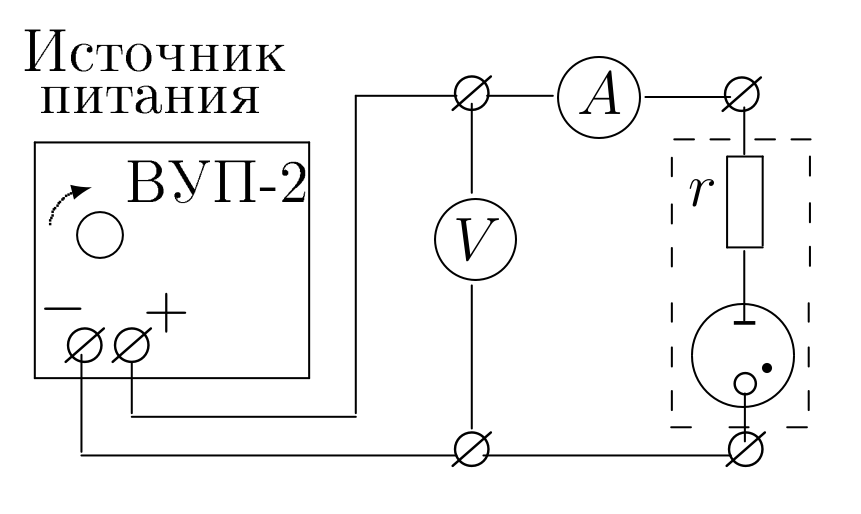
\includegraphics[scale = 0.2]{Workplace1}
    \centering
    \caption{Схема установки для изучения характеристик стабилитрона}
    \label{shem1}
\end{figure}

\begin{figure}[!h]
    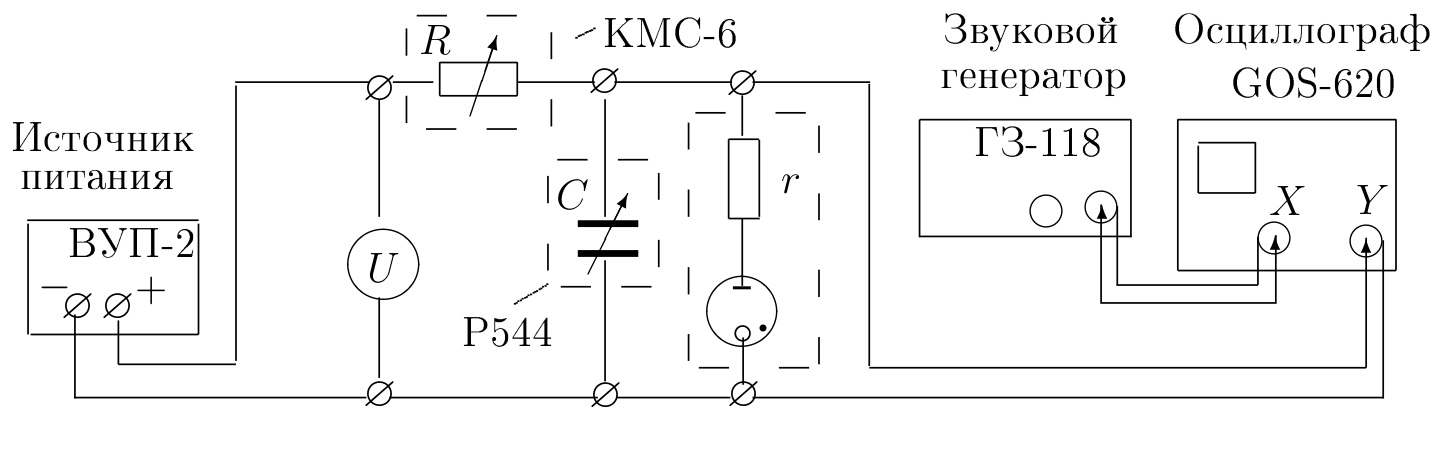
\includegraphics[scale = 0.2]{Workplace2}
    \centering
    \caption{Схема установки для исследования релаксационных колебаний}
\end{figure}

\parag {Ход работы} ~\\

\point Соберём схему по \ref{shem1}, выполним необходимые действия для подготовки к работе.

\point Снимем вольтамперную характеристику стабилитрона с резистором $r = 5,4$ кОм.

\begin{table}[!h]
    \centering
    \begin{tabular}{|c|c||c|c|}
        \hline
        \multicolumn{2}{|c||}{При возрастании} & \multicolumn{2}{c|}{При убывании} \\ \hline
        $I$, мА & $U$, В & $I$, мА & $U$, В  \\ \hline
        0 & 91 & 6.48 & 108.37 \\ \hline
        3.37 & 91.25 & 6.26 & 106.48 \\ \hline
        3.72 & 93.25 & 5.92 & 105.1 \\ \hline
        4.01 & 94.93 & 5.52 & 103.02 \\ \hline
        4.47 & 97.53 & 5.34 & 102.05 \\ \hline
        4.76 & 99.15 & 4.87 & 99.25 \\ \hline
        5.25 & 102.05 & 4.64 & 98.05 \\ \hline
        5.47 & 103.33 & 3.8 & 93.55 \\ \hline
        5.78 & 105.12 & 3.5 & 92.02 \\ \hline
        6.28 & 107.15 & 3.22 & 90.25 \\ \hline
        6.48 & 108.37 & 2.76 & 87.67 \\ \hline
            &        & 2.26 & 84.97 \\ \hline
            &        & 1.41 & 80.52 \\ \hline
            &        & 0 & 75.4 \\ \hline
    \end{tabular}
    \caption {Зависимость $U (I)$ при возрастании и убывании}
    \label{V-A}
\end{table}

Из таблицы видно, что, $V_1 = 91,25$ В, $I_1 = 3,37$ мА, $V_2 = 80,52$ В, $I_2 = 1,41$ мА.

\point Теперь соберём релаксационный генератор. Установим $C = 50$ нФ, $R = 0,9$ МОм. Выставим напряжение $U = 1,2 \cdot V_1 \approx 110$ В. Настроим осциллограф.

\point Получим пилу на экране. Оценим время зарядки и разрядки: $\tau_з \approx 60$ мс, $\tau_р \approx 5$ мс. Картину колебаний см. ниже на \ref{saw}.

\begin{figure}[!h]
    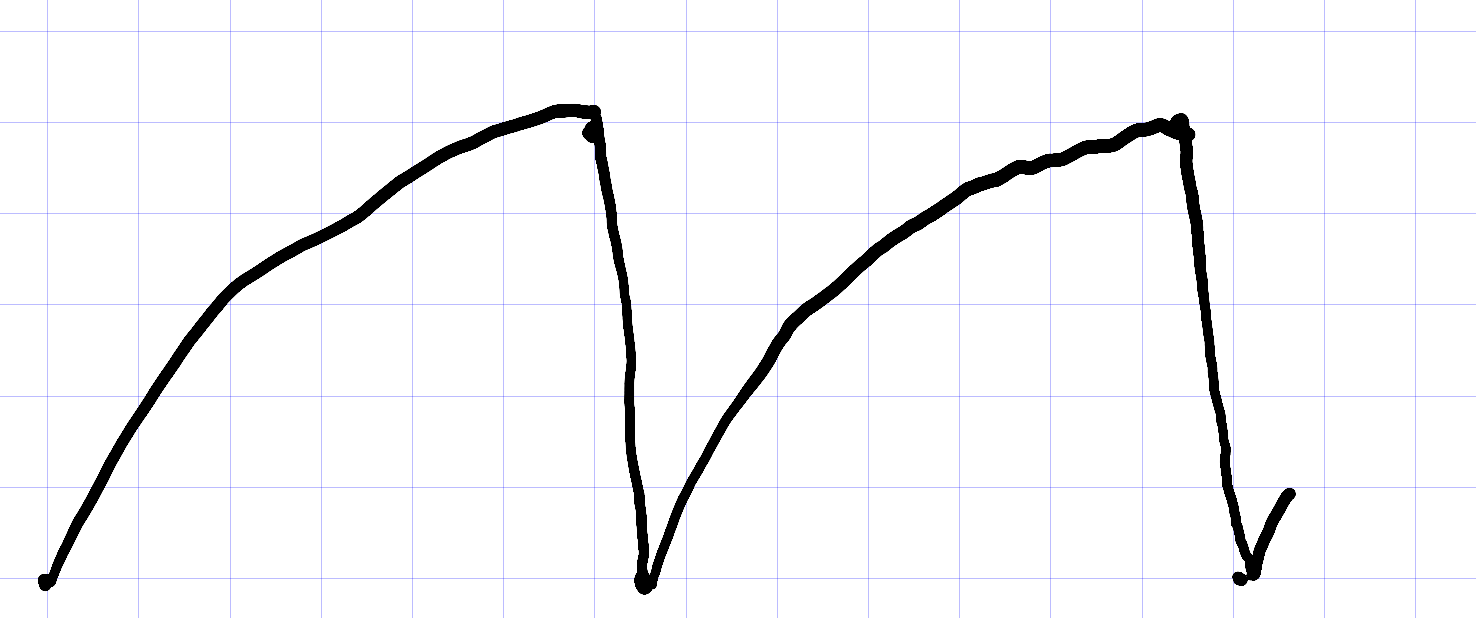
\includegraphics[scale = 0.2]{saw}
    \centering
    \caption{Картина колебаний для пилы}
    \label{saw}
\end{figure}

\point Найдём $R_{кр}$, при котором пропадают колебания. Убедимся, что при $R > R_{кр}$ (но не намного) и увеличении $U$ колебания также пропадают.

Получим: $R_{кр} = 1,4 \cdot 10^5$ Ом. По формуле же можно найти:

\[
    R_{кр} = \frac{U - V_2}{I_2} \approx 0,2 \cdot 10^5~Ом
\]

Такую большую разницу можно объяснить тем, что $V_2$ и $I_2$ были измерены неточно.

\point Восстановим исходные параметры релаксационного генератора. Получим фигуры Лиссажу, соответствующие соотношению частот 1:1, 2:1, 3:1. Получаем следующие изображения (см. таблицу \ref{liss}):

\begin{table}[!h]
    \begin{tabular}{ccc}
        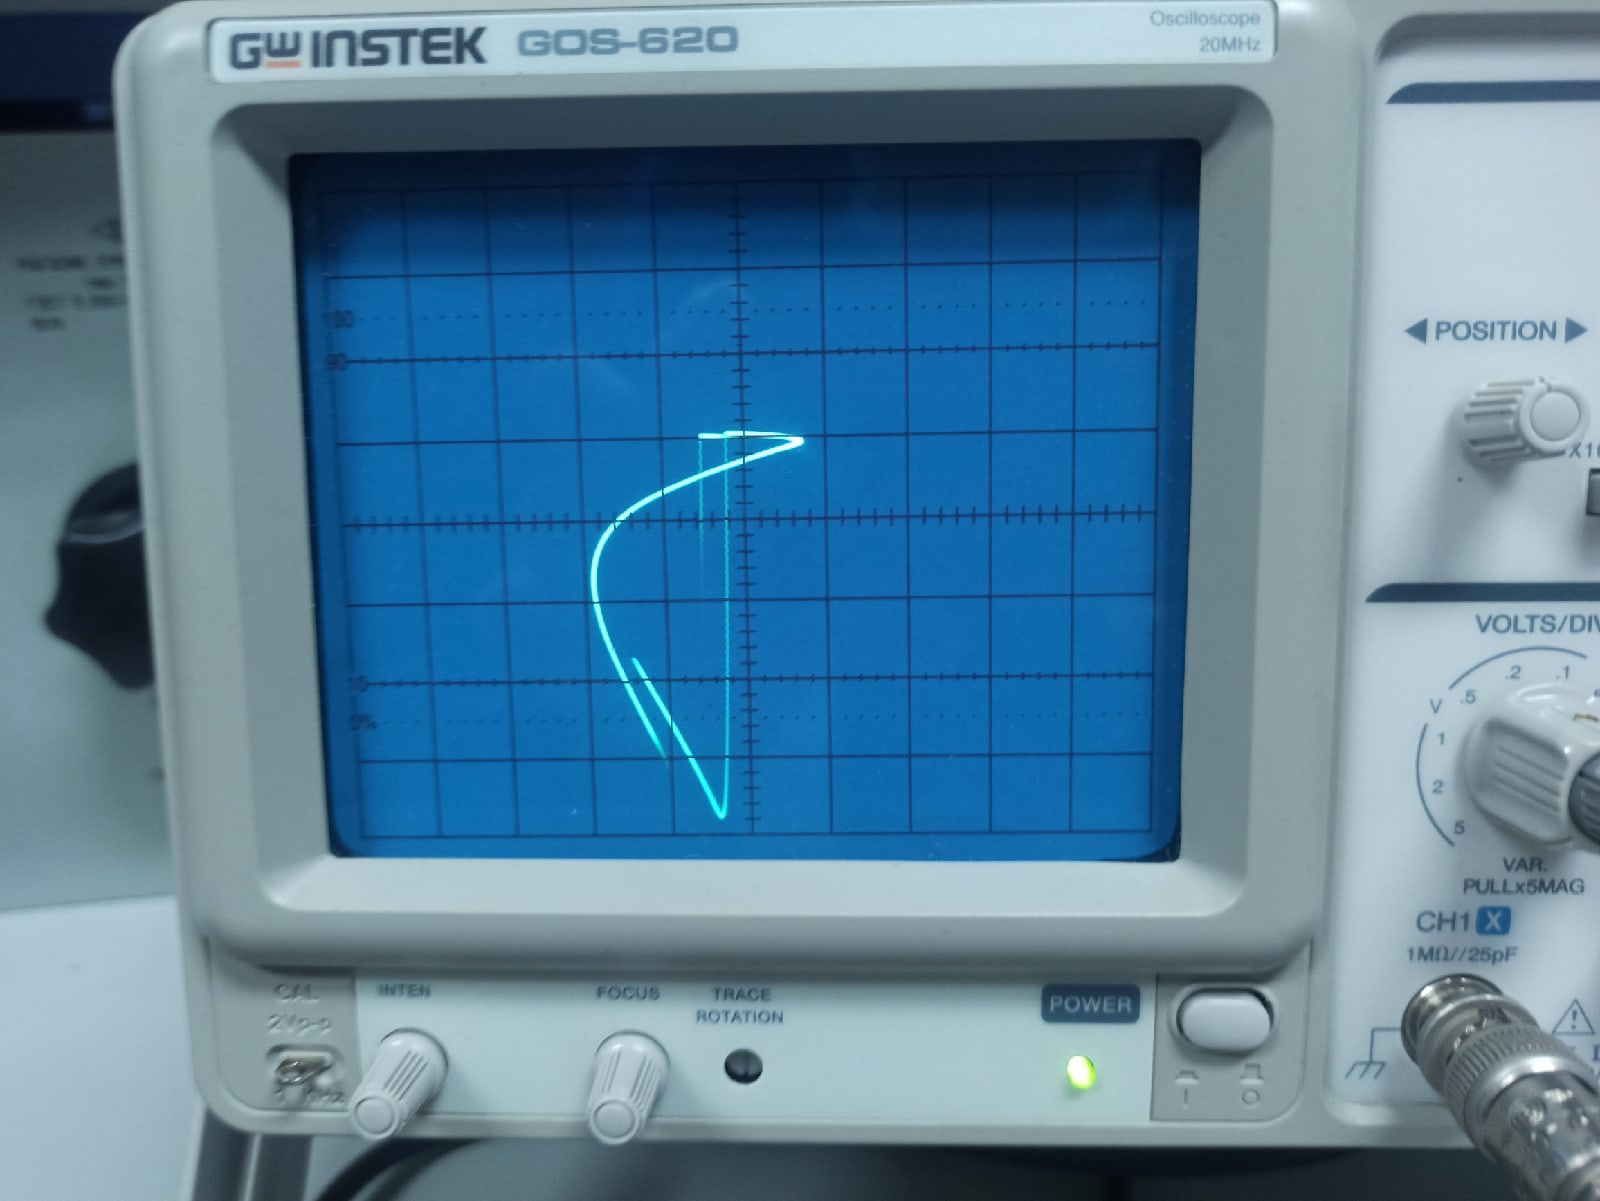
\includegraphics[scale = 0.1]{0int} &
        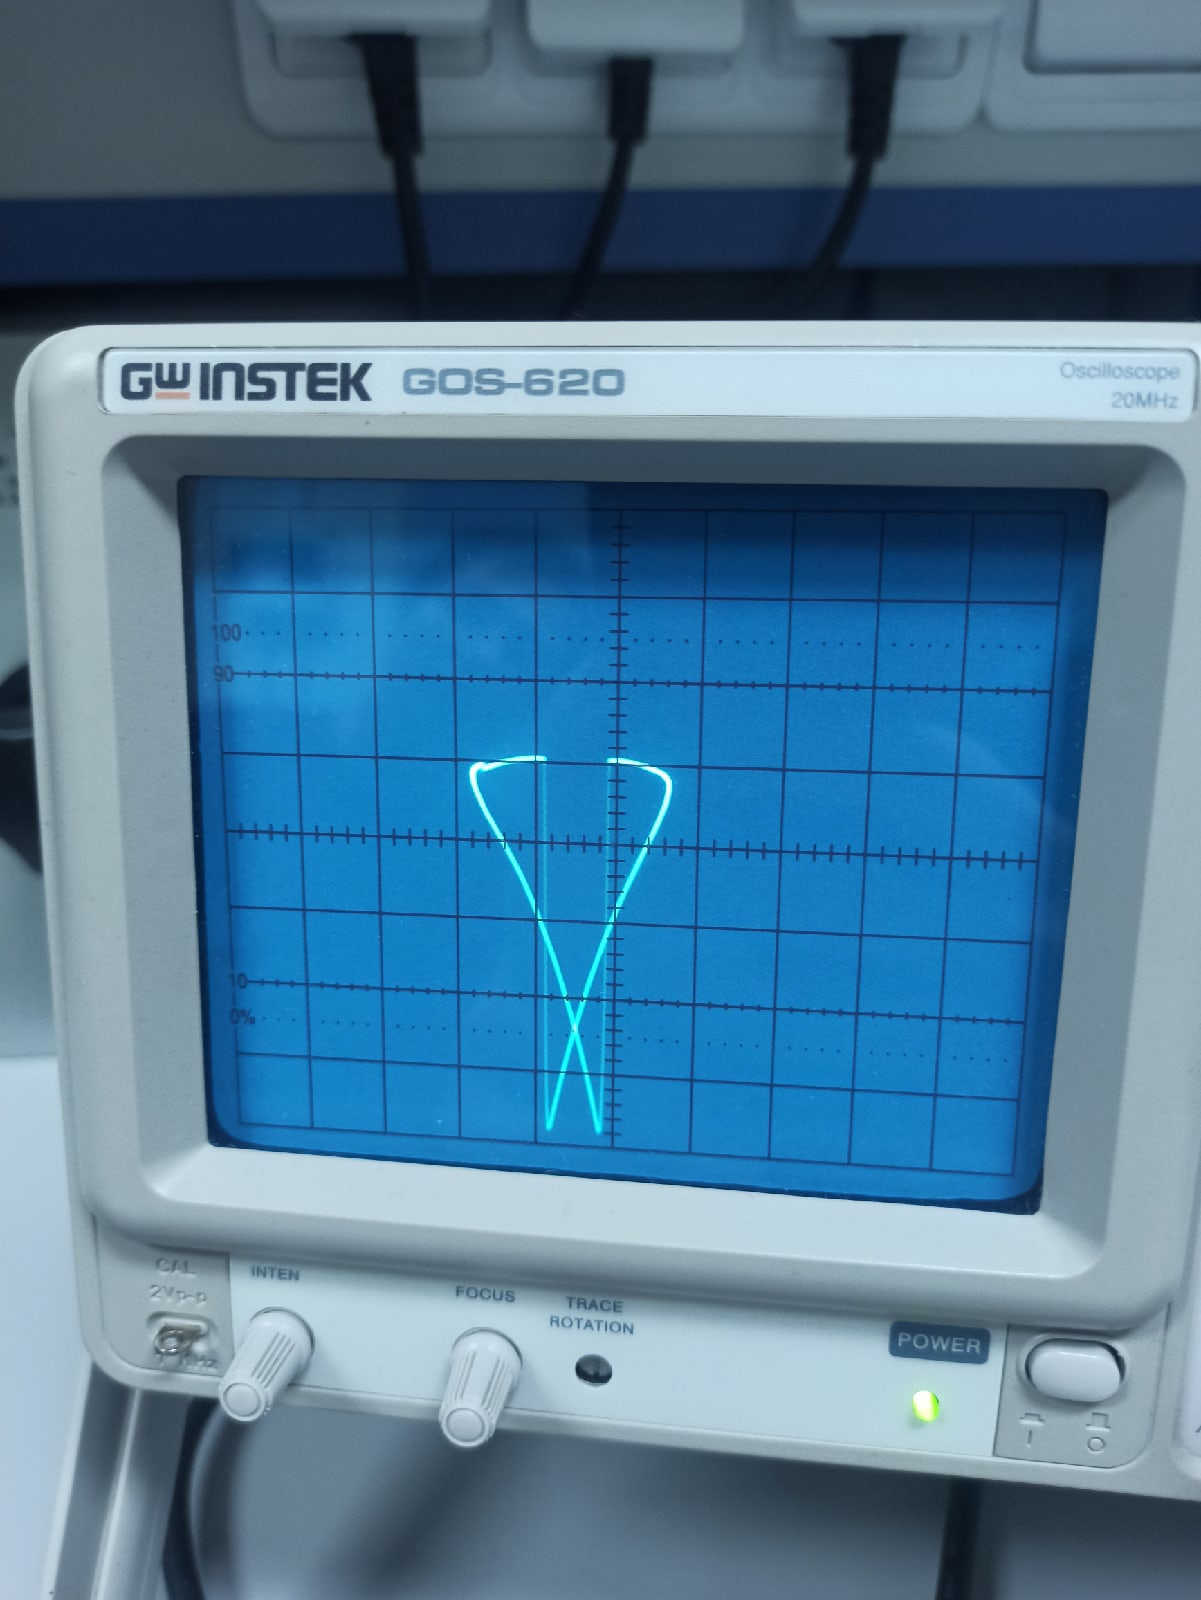
\includegraphics[scale = 0.1]{1int} &
        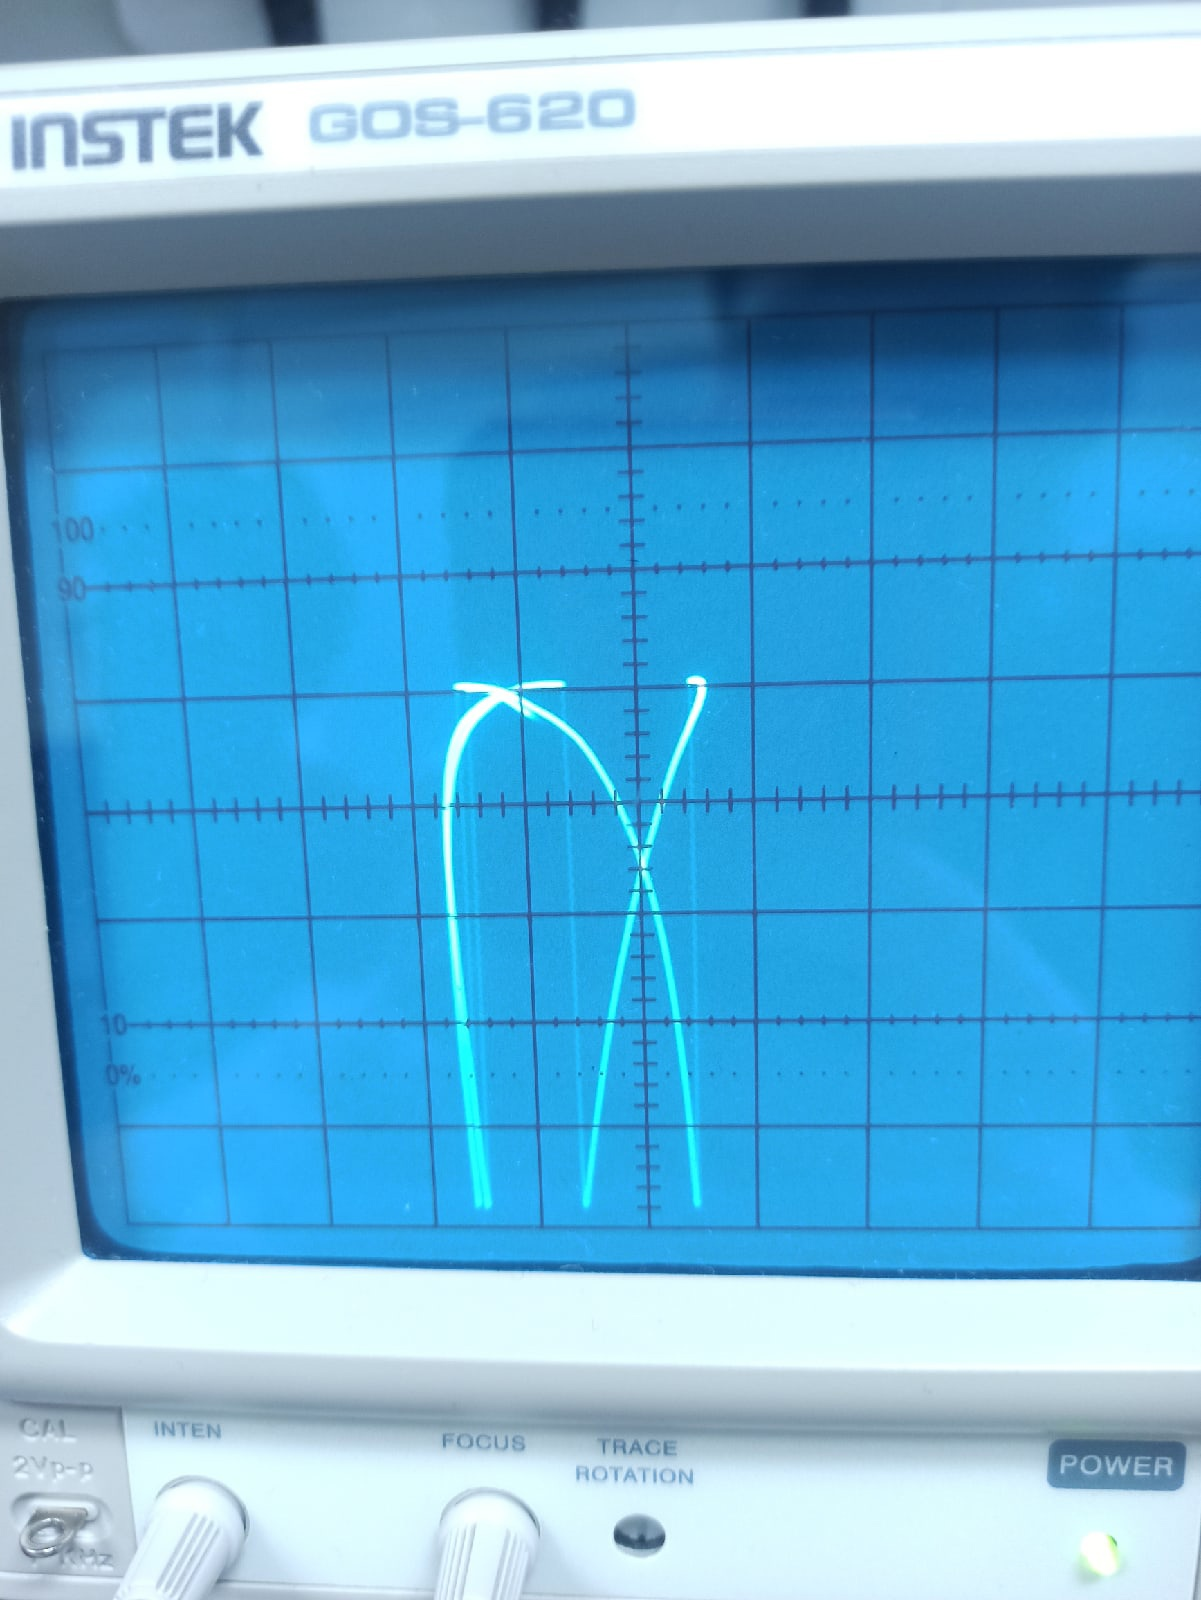
\includegraphics[scale = 0.1]{2int} \\
        1:1 &
        2:1 &
        3:1
    \end{tabular}
    \caption {Фигуры Лиссажу}
    \label {liss}
\end{table}

\point При $R = 5,2 \cdot 10^5$ Ом снимем зависимость зависимость $f (C)$ с помощью фигур Лиссажу 1:1. Результаты см. в таблице \ref{fC}.

\begin{table}[!h]
    \centering
    \begin{tabular}{|c|c|c|c|c|c|}
        \hline
        $f$, Гц & 150 & 75 & 50 & 37 & 30\\ \hline
        $С$, мкФ & 0.01 & 0.02 & 0.03 & 0.04 & 0.05
        \\ \hline
    \end{tabular}
    \caption {Зависимость $f (C)$}
    \label{fC}
\end{table}

\point При $C = 10$ нФ снимем зависимость $f (R)$ с помощью фигур Лиссажу 1:1. Результаты см. в таблице \ref{fR}.

\begin{table}[!h]
    \centering
    \begin{tabular}{|c|c|c|c|c|c|c|c|c|}
        \hline
        $f$, Гц & 17 & 19 & 22 & 25.7 & 31 & 39.5 & 53 & 78.2\\ \hline
        $R, 10^5$ Ом & 9 & 8 & 7 & 6 & 5 & 4 & 3 & 2
        \\ \hline
    \end{tabular}
    \caption {Зависимость $f (R)$}
    \label{fR}
\end{table}

\parag {Обработка результатов} ~\\

\point По таблице \ref{V-A} построим графики вольтамперной характеристики в случае возрастания и убывания.

\begin{figure}[!h]
    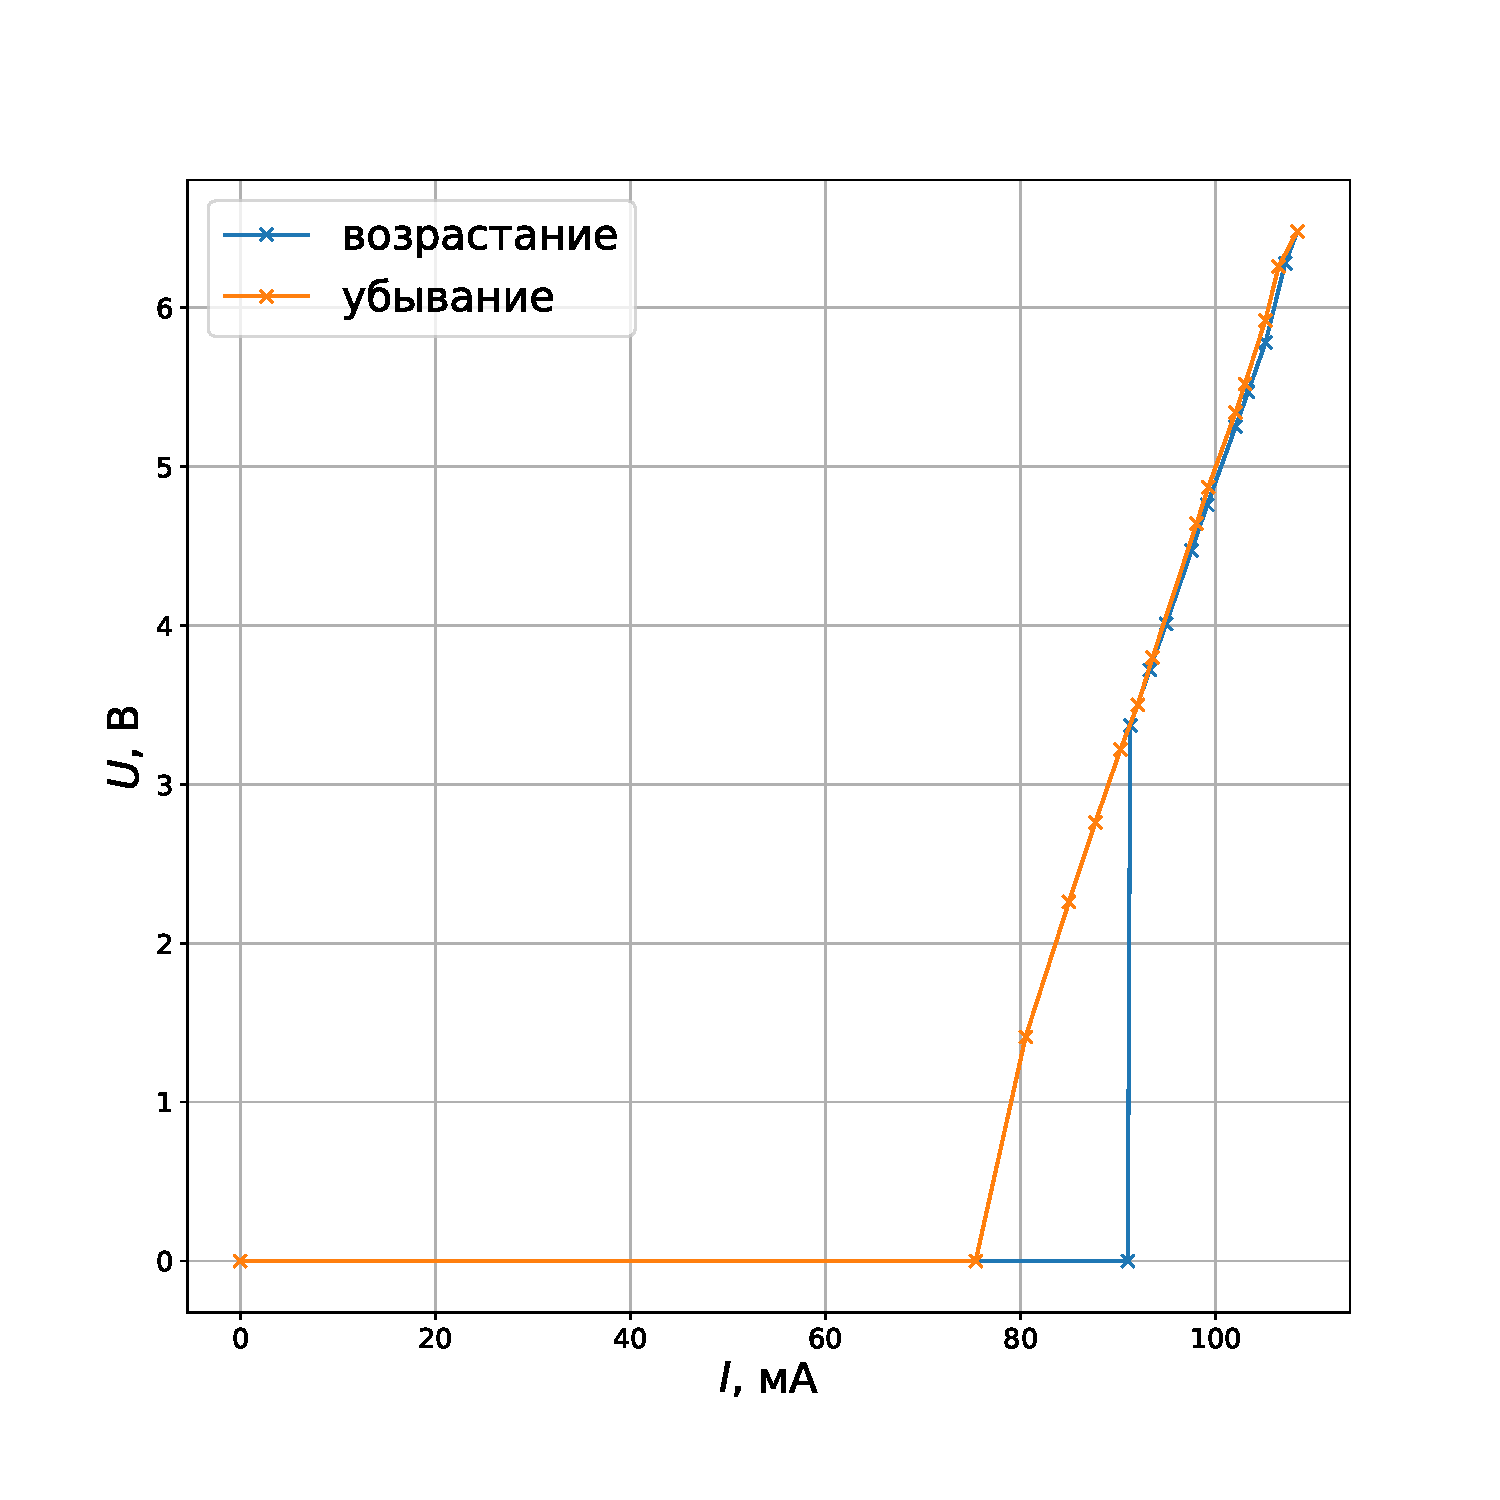
\includegraphics[scale = 0.365]{V_A}
    \centering
    \caption{Вольтамперная характеристика}
    \label{V-A}
\end{figure}

Теперь построим график только с возрастанием, но для сравнения проведём график, в котором не учитывается падение напряжения на $r$. Результат представлен на рисунке \ref{V-A-r}.

\begin{figure}[!h]
    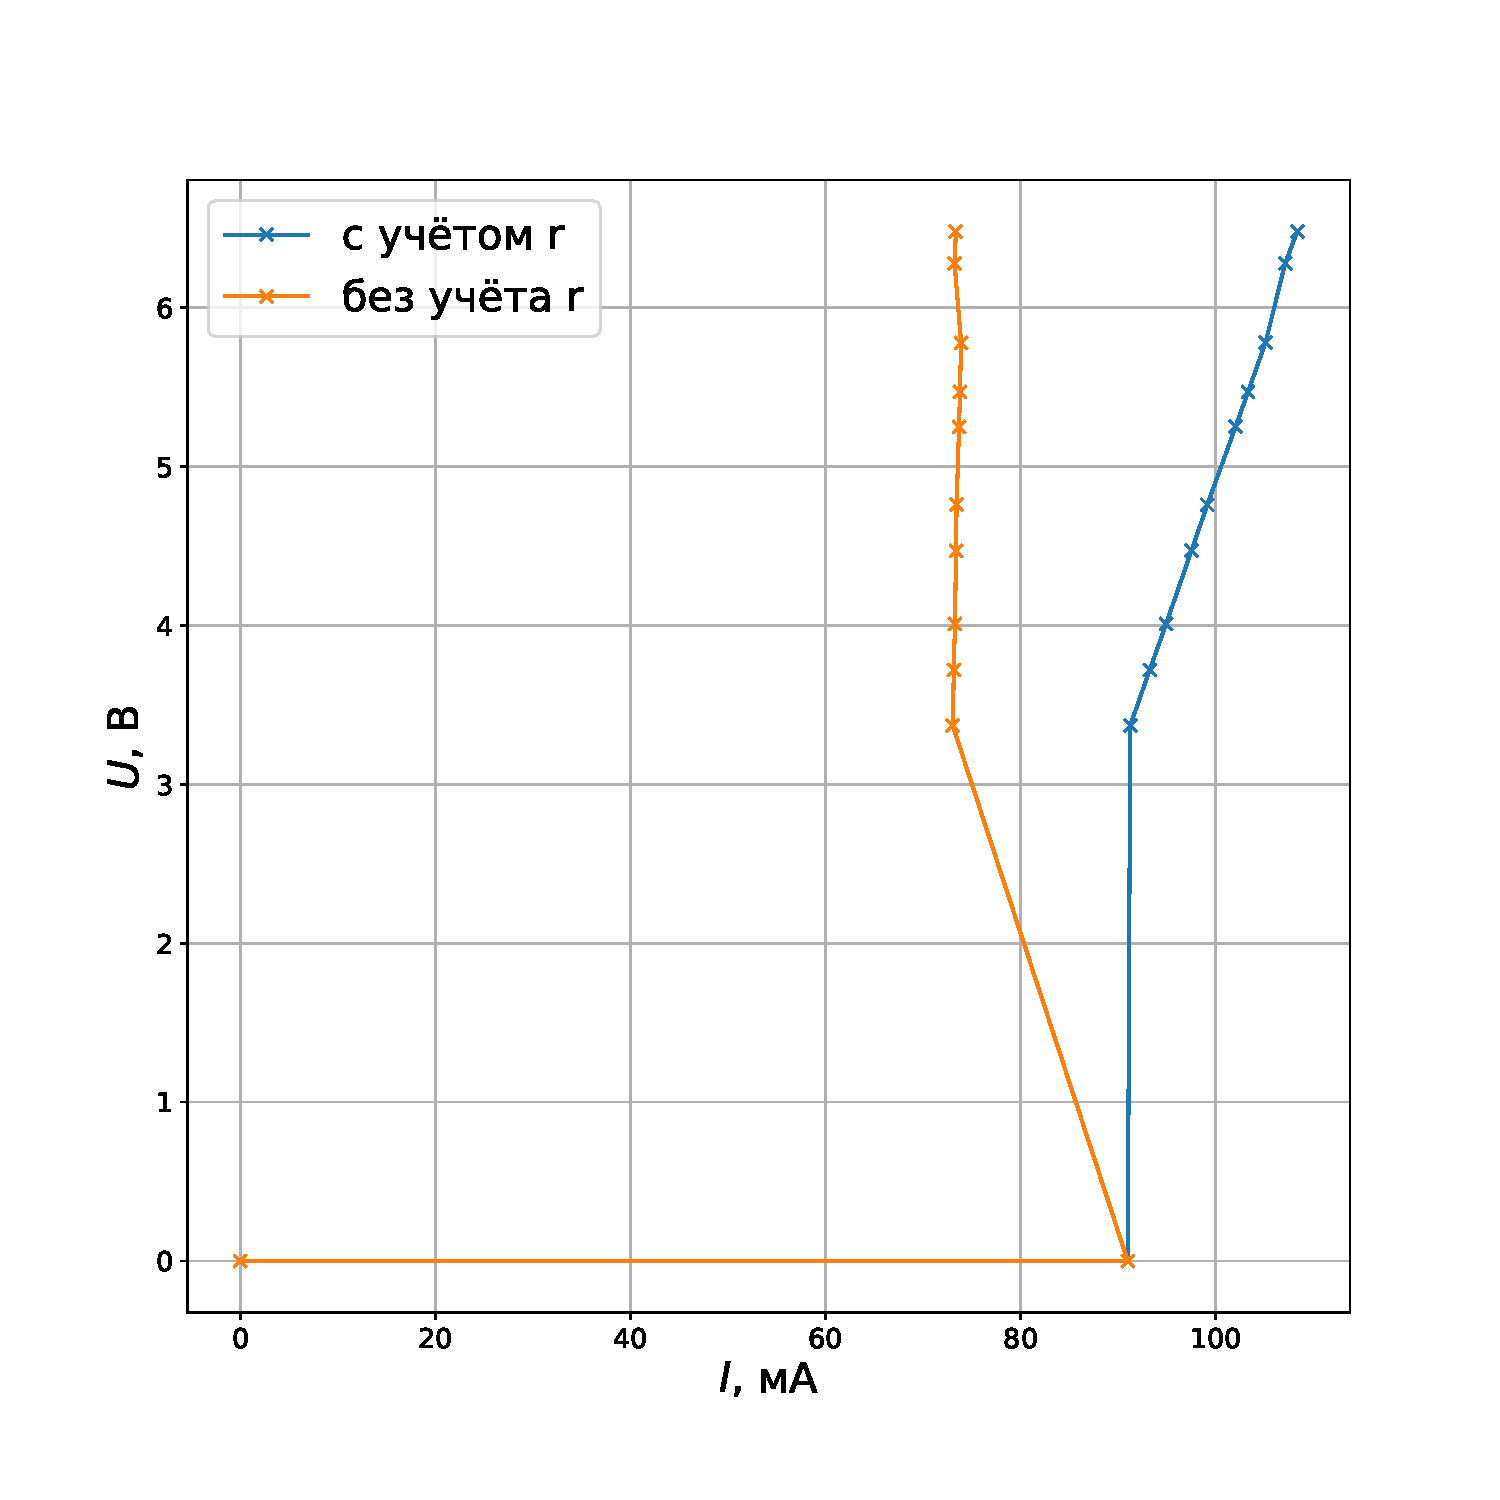
\includegraphics[scale = 0.365]{V_A_r}
    \centering
    \caption{Вольтамперная характеристика в сравнении}
    \label{V-A-r}
\end{figure}

\point Построим графики $T_{эксп} (C)$ и $T_{теор} (C)$ согласно таблице \ref{fC}. Результаты см. на рисунке \ref{T_C}.

\begin{figure}[!h]
    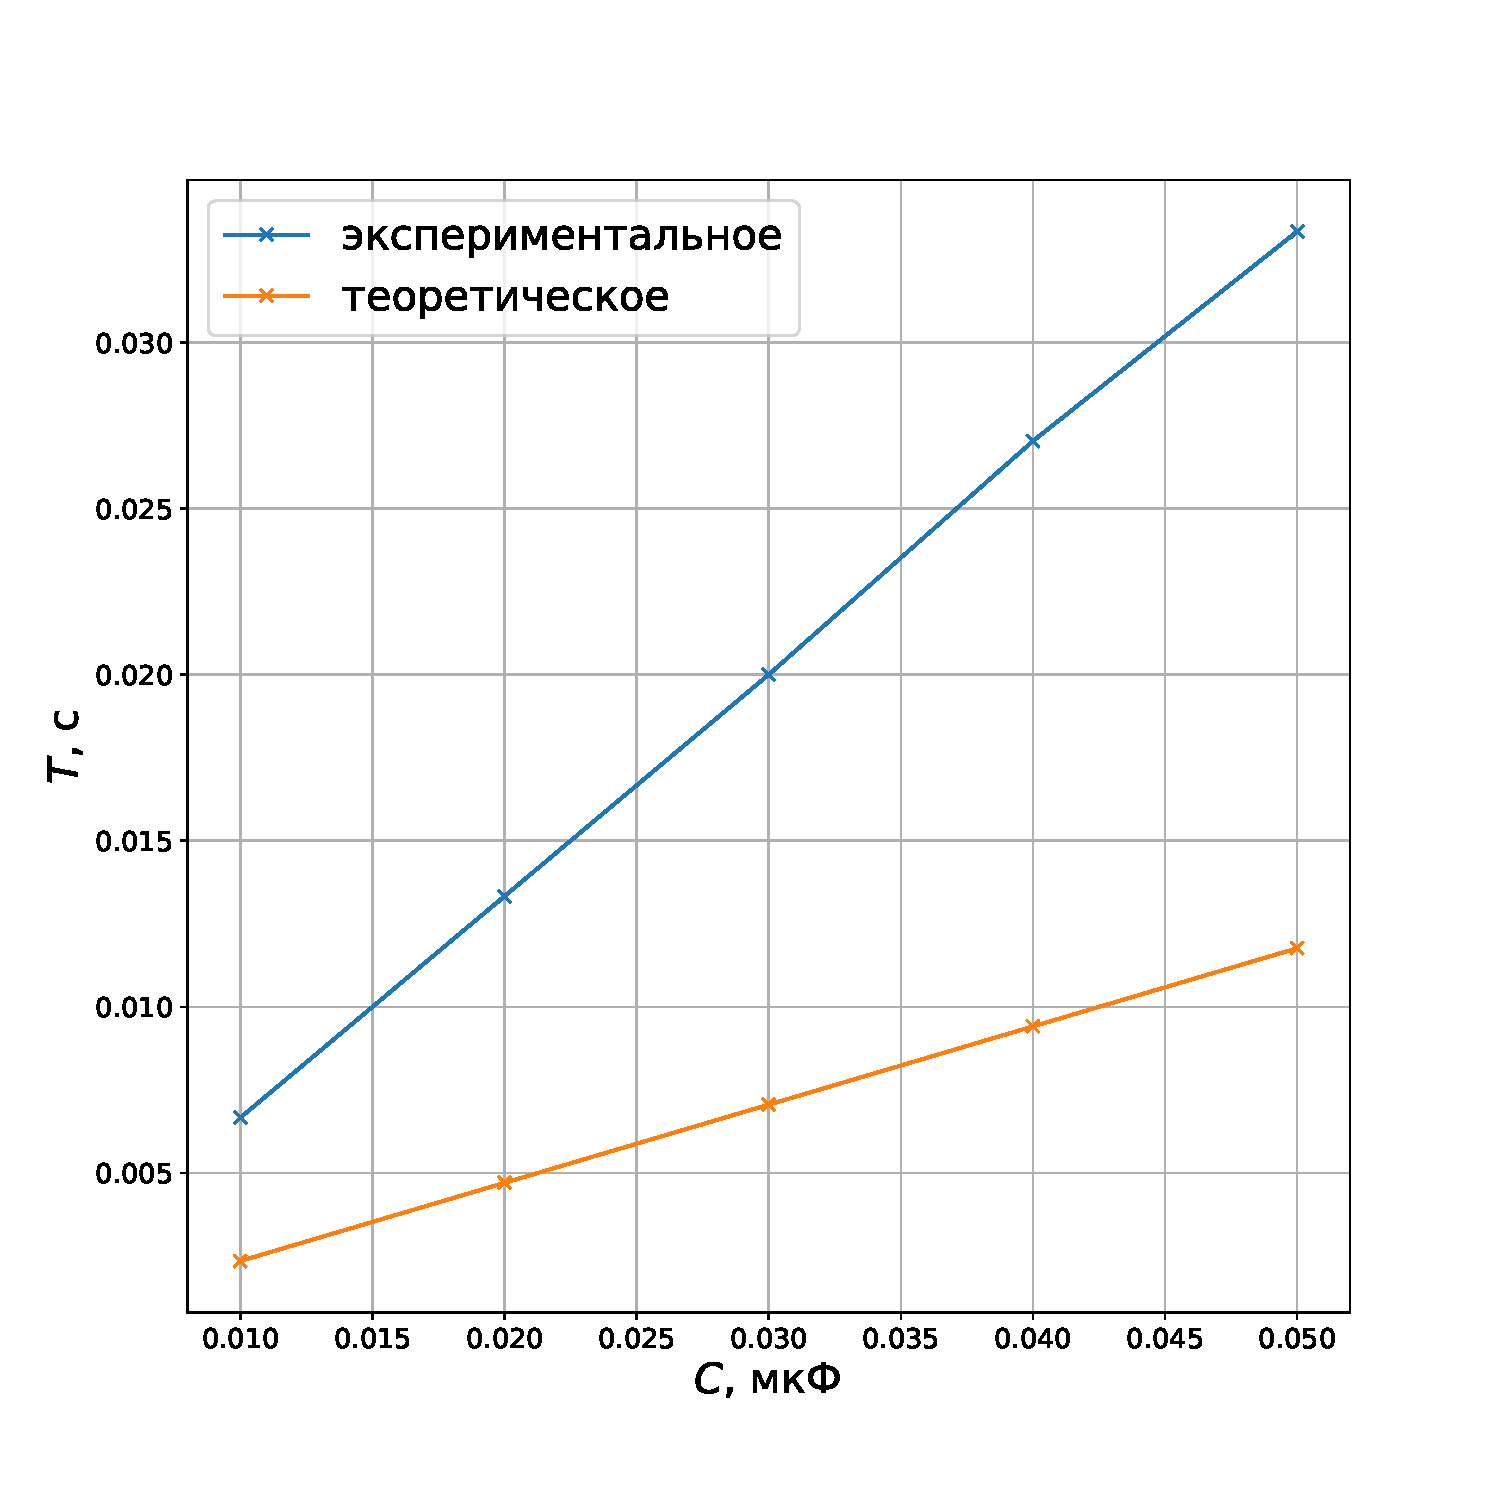
\includegraphics[scale = 0.365]{T_C}
    \centering
    \caption{Зависимость периода от ёмкости}
    \label{T_C}
\end{figure}

\point Построим графики $T_{эксп} (R)$ и $T_{теор} (R)$ согласно таблице \ref{fR}. Результаты см. на рисунке \ref{T_R}.

\begin{figure}[!h]
    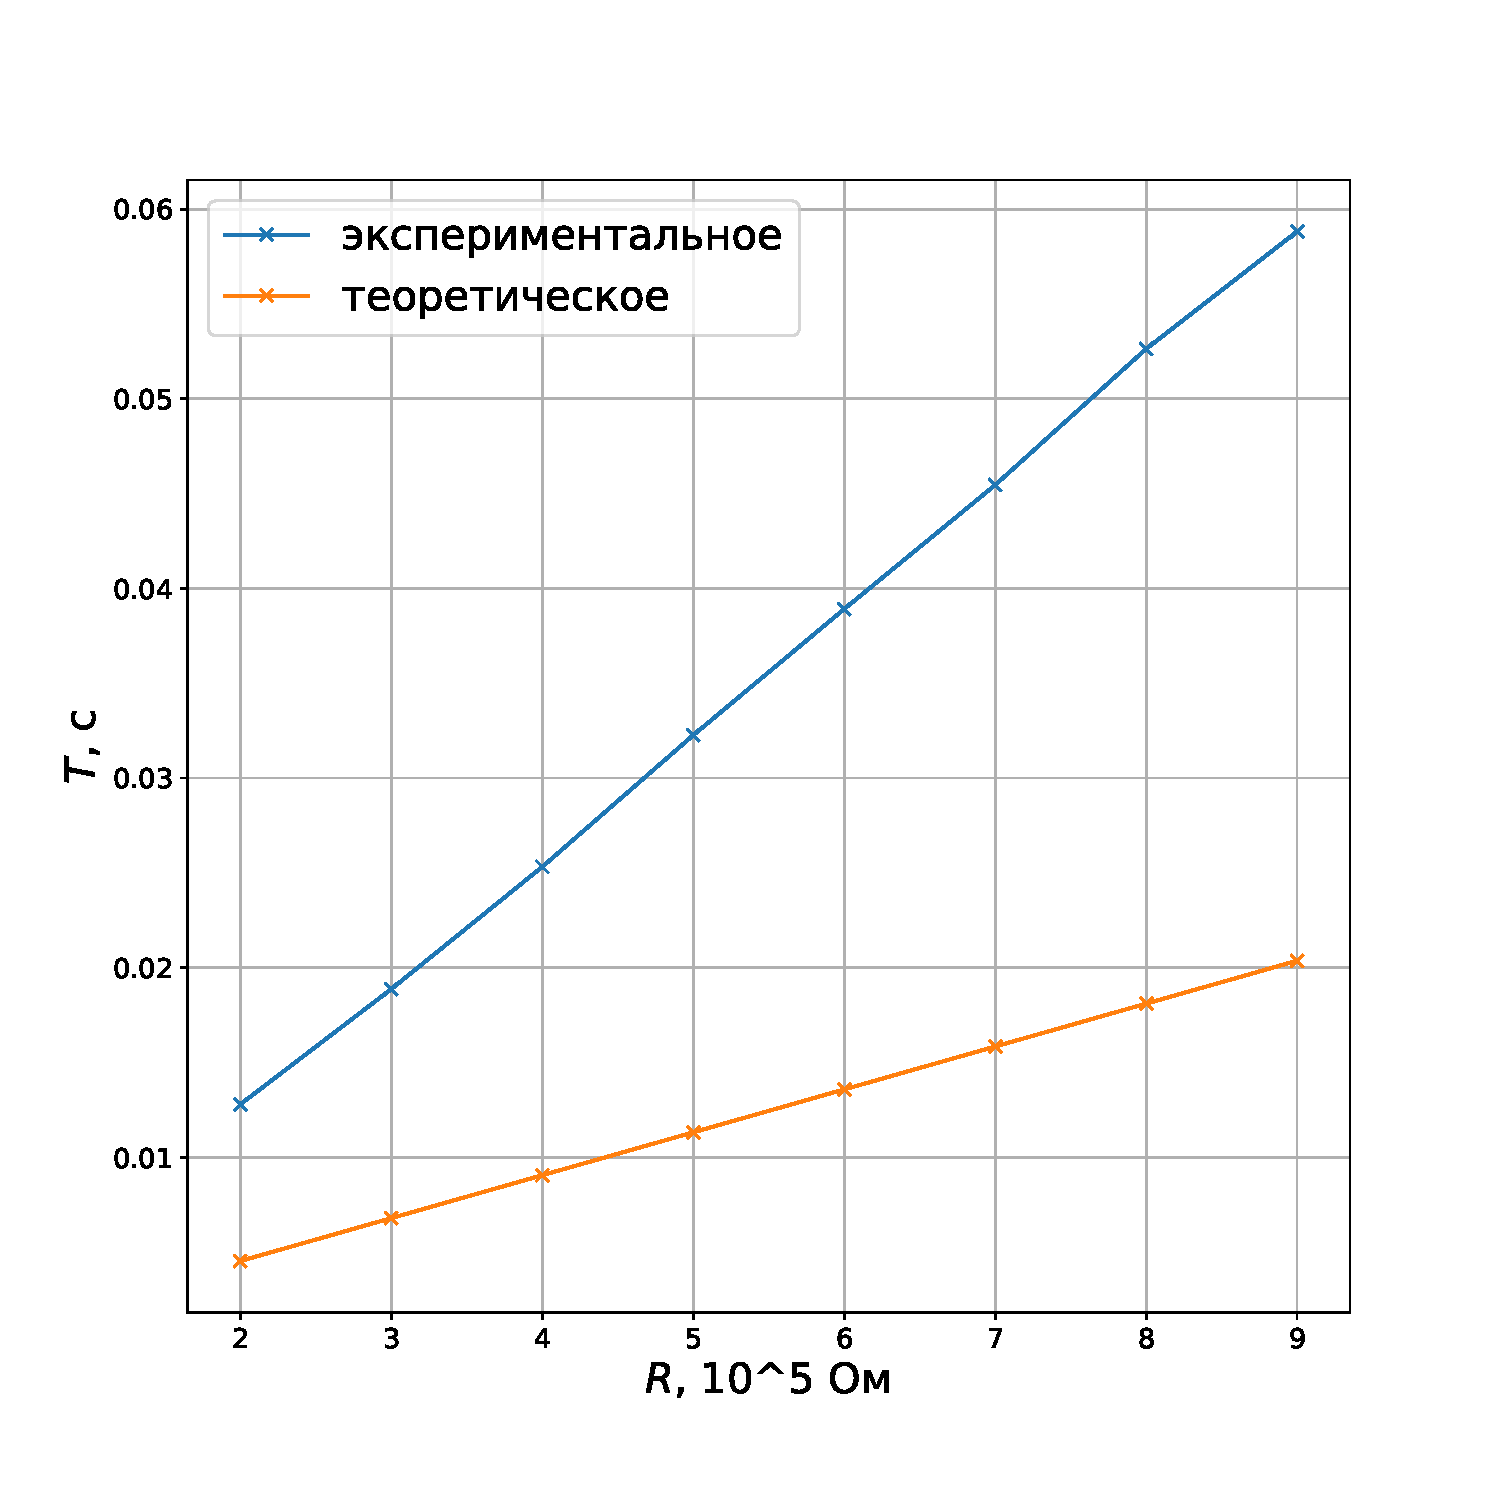
\includegraphics[scale = 0.365]{T_R}
    \centering
    \caption{Зависимость периода от ёмкости}
    \label{T_R}
\end{figure}

\end {document}
